

\graphicspath{{./ch_LDE_SI/figures/}}

\chapter{Heralded entanglement}



\subsection{Setup}
We perform the experiments with two home-built low-temperature confocal microscopes. Each setup features lasers for off-resonant and resonant excitation, cryogenic piezoelectric positioners and high-efficiency/low background fluorescence detection paths. The zero-phonon line (ZPL) detection paths of both setups lead to the common beam splitter and photon detectors used for the entanglement generation. Each setup has an independent microwave (MW) source (Rohde \& Schwarz SMB100A) and MW amplifier (Amplifier Research 20S1G4 and AR 40S1G4 for setups A and B, respectively) to drive the NV centre electron spins.

Sample A is mounted on a XYZ stepper/scanner piezo stack (Attocube) in a Janis ST-500 flow cryostat and kept at $T \approx 8$\,K. Sample B is mounted on a XYZ stepper (Attocube) inside a custom-built Cryovac bath cryostat with optical access and kept at a temperature of $T \approx 4$\,K. 

Off resonant green excitation is provided for each of the setups by 532\,nm lasers (Spectra Physics Millenia Pro and Laser 2000 Cobalt Samba for setups A and B, respectively). Two tuneable 637\,nm lasers (New Focus Velocity) for independent resonant excitation are used for optical spin-pumping. For  the resonant excitation pulses used to generate the entanglement both setups share a tuneable continuous wave 637\,nm laser (Sirah Matisse DS). Its output is sequentially fed through an acousto-optic modulator (AOM; Crystal Technologies) and an electro-optic modulator (EOM; Jenoptik). After passing through the AOM \& EOM, the beam is split using a 50/50 beam splitter, and a 30 cm adjustable delay line is inserted in one arm for fine-tuning the temporal overlap of the excitation.

The photon emission of each NV is split into a ZPL part and an off-resonant phonon sideband (PSB) part by a dichroic long-pass filter (Semrock LPD01-633RS). The PSB emission is independently detected for each setup by avalanche photo-diodes (APDs; Perkin-Elmer SPCM). The ZPL emission is further filtered by a second dichroic filter (to remove green excitation light) and a tuneable band pass filter (Semrock TBP-700B). After filtering resonant excitation light by cross-polarisation rejection the ZPL emission of NVs A and B is coupled into the input ports of a fibre-coupled beam splitter (Evanescent Optics) by polarisation-maintaining fibres. The photons leaving the output ports of the beam splitter are detected by fibre-coupled avalanche photo-diodes (Picoquant Tau-SPAD) and time-tagged by a Picoquant Hydraharp 400 system.

\subsection{Rejection of resonant excitation light}
The experimental protocol requires the resonant excitation of a single optical transition and the detection of indistinguishable resonant photons from spontaneous emission of this transition. We use polarisation rejection and time-filtering to filter residual resonant excitation light --- stemming from reflections from optical elements and the sample surface --- from the signal.

The excitation laser is linearly polarised and rotated using a half-wave-plate (HWP) to a non-zero angle $\varphi$  with respect to the (linear) dipole of the $\ket{\up}\leftrightarrow\ket{E_y}$ transition it excites (Fig.\,\ref{fig:resonant_detection}). In the detection path, the combination of a half-wave plate and polariser sets a detection axis with an angle $\theta$ in the opposite direction with respect to the NV transition dipole. A further quarter-wave-plate (QWP) corrects for circular polarisation components of the signal that are induced by optical elements in the detection path.  We find the optimum in laser-rejection, NV excitation efficiency and NV collection efficiency by varying the angles $\varphi,\theta$ while keeping $\varphi + \theta = 90^\circ$.
% $\varphi=\theta=45^\circ$ will reject the laser reflections while reducing the NV collection efficiency by half.

As can be seen in Fig.\,\ref{fig:laser_vs_nv}, reflections of the two-nanosecond excitation pulse can be clearly distinguished from the exponentially decaying NV centre emission. In this manner laser reflections that are not removed by the polarisation rejection can be removed by time-filtering. %We note that because of the detector dead-time it is only possible to detect one photon per excitation pulse, therefore a combination of polarisation rejection and time filter is required. 
\begin{figure}[h]
\centering
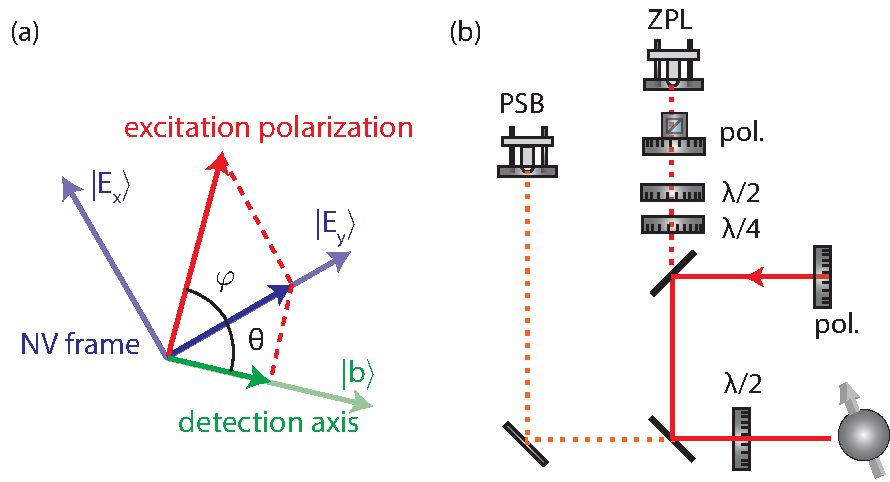
\includegraphics[width=10cm]{resonant_excitation_detection_gerwin.pdf}
\caption{Resonant detection and excitation. \textbf{a}, Working principle of cross-polarisation rejection. \textbf{b}, Optical setup. See text for details.}
\label{fig:resonant_detection}
\end{figure}

\subsection{Experimental control}
For the experiment to be feasible, a high repetition rate of the entanglement generation sequence is crucial, because the success probability per shot is small, $P_\mathrm s = 1/2 \times \eta_\mathrm A\eta_\mathrm B \approx 10^{-7}$. We achieve a reasonable repetition rate by employing a conditional protocol as follows (Fig.\,\ref{fig:conditional_measurement}): We first ensure that both NV centres are in the negative charge state and on resonance. To this end we independently re-set the charge and resonance state of the two NVs with green laser pulses until the resonant excitation lasers are on resonance \cite{Robledo:2011fs,Pfaff:2012ue}. After this preparation we run the spin-preparation and entanglement generation sequence. In case of successful generation of entanglement we read out both spins in a single shot and return to the charge and resonance (CR) check. Otherwise, we repeat spin-preparation and entanglement generation. After 300 unsuccessful entanglement attempts we start over with the CR check. The success probabilities for passing the CR check, $P_\mathrm{CR} \approx 2\%$, and for successfully generating entanglement let us predict an entanglement generation rate of $\sim 1/10\,\mathrm{minutes}$. For comparison, an unconditional protocol in which charge/resonance and entanglement generation are only verified in post-processing would yield an entanglement rate of only $\sim 1/50\,\mathrm{hours}$.

\begin{figure}[h]
\centering
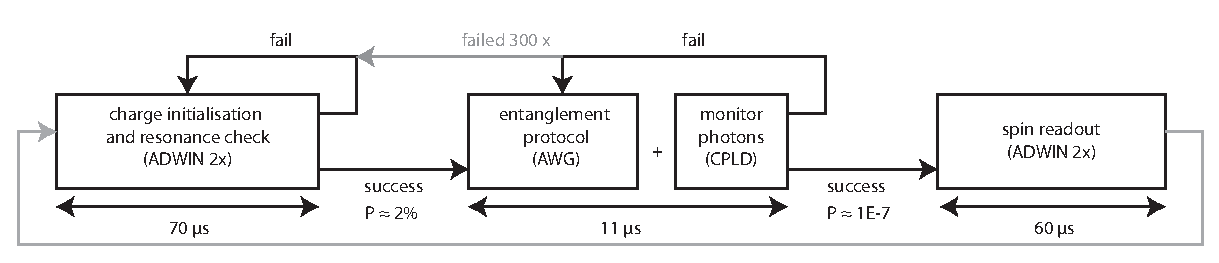
\includegraphics[width=\textwidth]{conditional.pdf}
\caption{The conditional sequence to implement the entanglement protocol. Two programmable micro-controllers with integrated DAC- and counter modules ({\em ADwin 2x})  independently initialise each NV centre and perform the charge-resonance check described in the main text. If both checks pass, a trigger is sent to the Arbitrary Waveform Generator ({\em AWG}) that executes the entanglement protocol. The protocol is run up to 300 times until it is successful. A successful attempt is recognised by a logic device ({\em CPLD}) that looks for a success-signature in the stream of photon clicks produced, and sends a halt trigger to the AWG when it does. The readout is then performed by the ADwins, after which the sequence starts over.}
\label{fig:conditional_measurement}
\end{figure}

Conditional operation is implemented in the following manner: The CR check and readout is done independently for the two setups by two programmable micro-controllers with DAC- and counter modules (Adwin Gold II and Adwin Pro II for setup A and B, respectively). Once both CR checks pass, a start trigger is sent to the Arbitrary Waveform Generator (Tektronix AWG 5014C) that sequentially executes the entanglement protocol up to 300 times. For each round, the photon clicks are recorded and time-tagged by a Picoquant Hydraharp 400 system. In addition, the photon clicks are also monitored in real time by a programmable logic device (CPLD; Altera Max V development kit) that time-filters the signal and recognises a successful entanglement event; if a success occurs, a stop trigger is sent to the AWG within 50\,ns to prevent it from running the next entanglement cycle. Furthermore, the logic device triggers both ADwin micro controllers to start their readout sequence. Further (more selective) time filtering is done in post-processing for the successful events, by combining the time-tagged data and spin readout data.

\subsection{Optical Rabi oscillations}
On resonance (i.e. in the absence of quasi-static spectral diffusion), the exponential damping time $\tau_{\text{rabi}}$ of the Rabi oscillations is determined by the pure optical dephasing time $T_2^{*,\text{opt}}$ via\cite{Robledo2010}
\be
\frac{1}{\tau_{\text{rabi}}}=\frac{3}{4 T_1} + \frac{1}{2T_2^{*,\text{opt}}},
\ee
where $T_1$ is the NV centre optical lifetime (about 12 ns).

As can be seen in Fig.\,2b in the main text, and Fig.\,\ref{fig:cr_nv_B}, $\tau_{\text{rabi}}$ saturates to the lifetime-limited value for high thresholds. Similar saturation behaviour is observed for different optical Rabi frequencies.

\begin{figure}[h]
\centering
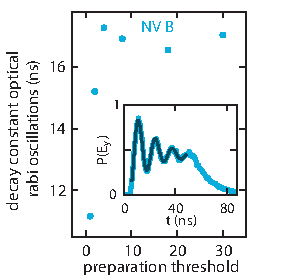
\includegraphics[width=5cm]{cr_NV_B.pdf}
\caption{Line-narrowing effect of the dynamical initialization of charge and resonance for NV B, exemplified by the dependence of the decay time of optical Rabi oscillations on preparation threshold. See Fig.\,2b in the main text for details of the pulse sequence used.}
\label{fig:cr_nv_B}
\end{figure}


\section{Fidelity measure}

We want to estimate the fidelity of the generated two-spin state $\ket{\psi}$ with respect to the ideal Bell state. We take the example of the Bell state $\Psi^+$:
\begin{equation}
\ket{\Psi^+} = (\ket{\uparrow}_\mathrm{A}\ket{\downarrow}_\mathrm{B} + \ket{\downarrow}_\mathrm{A}\ket{\uparrow}_\mathrm{B})/\sqrt{2} \equiv (\ket{\uparrow\downarrow}+\ket{\downarrow\uparrow})/\sqrt{2} ,
\end{equation}
where $\ket{\uparrow}$ and $\ket{\downarrow}$ denote the $\mszero$ and $\msmone$ spin sub-levels of the NV centre ground state and subscripts A, B indicate the two NV centres used. The density matrix for this state is
\begin{equation}
\rho_{\Psi^+} = \ket{\Psi^+}\bra{\Psi^+} = \frac{1}{2}\left(
\begin{array}{cccc}
 0 & 0 & 0 & 0 \\
 0 & 1 & 1 & 0 \\
 0 & 1 & 1 & 0 \\
 0 & 0 & 0 & 0
\end{array}
\right).
\end{equation}
The fidelity of the state $\ket{\Psi^+}$ with density matrix $\rho$, for both spins in the z-basis, is therefore
\begin{equation}
\mathcal{F} = \bra{\Psi^+}\rho\ket{\Psi^+} = \frac{1}{2}(\rho_{22}+\rho_{33}+\Re(\rho_{23})+\Re(\rho_{32})) = \frac{1}{2}(\rho_{22}+\rho_{33}+ 2\Re(\rho_{23})).
\end{equation}
The term coming from the diagonal elements, $\rho_{22} + \rho_{33}$, is given by the fraction of spin-readouts in which the outcomes from NVs A and B are anti-correlated. To estimate the off-diagonal terms we measure both spins in the X-basis by applying $\pi/2$-rotations around $\mathbf y$, yielding the density matrix
\begin{equation}
\tilde{\rho} = \left ( \sqrt{Y}\otimes\sqrt{Y} \right ) \rho \left ( \sqrt{Y}^{\dagger}\otimes\sqrt{Y}^{\dagger} \right ),
\end{equation}
where the operator $Y$ describes a $\pi$-rotation around the y-axis, 
\be
\sqrt{Y} = \mathrm e^{-\frac{\mathrm i}{\hbar} S_\mathrm y \pi/2},
\ee
where $S_\mathrm y$ is the y-component of the spin-$\frac{1}{2}$ operator. The contrast between measured correlations and anti-correlations in this basis is
\begin{equation}
\tilde{\rho}_{11}+\tilde{\rho}_{44}-\tilde{\rho}_{22}-\tilde{\rho}_{33} = 2\Re(\rho_{23})+2\Re(\rho_{14}).
\end{equation}
It follows from the definition of the density matrix that the absolute of $\Re(\rho_{14})$ is bounded by
\begin{equation}
\mid \Re(\rho_{14}) \mid \leq \sqrt{\rho_{11}\rho_{44}},
\end{equation}
and therefore
\begin{equation}
2\Re(\rho_{23}) \geq \tilde{\rho}_{11}+\tilde{\rho}_{44}-\tilde{\rho}_{22}-\tilde{\rho}_{33} - 2\sqrt{\rho_{11}\rho_{44}}.
\end{equation}
In terms of measured quantities in two bases, the fidelity has thus a strict lower bound of\cite{Blinov2004a}
\begin{equation}
\label{eq:fidlowerbound}
\mathcal{F} \geq \frac{1}{2}\left(\rho_{22}+\rho_{33}+\tilde{\rho}_{11}+\tilde{\rho}_{44}-\tilde{\rho}_{22}-\tilde{\rho}_{33} - 2\sqrt{\rho_{11}\rho_{44}}\right).
\end{equation}
The treatment for the Bell state $\ket{\Psi^-} = (\ket{\uparrow\downarrow}-\ket{\downarrow\uparrow})/\sqrt{2}$ and for rotations around other axes is analogous. For the best estimate of the fidelity as mentioned in the main text, the term $\sqrt{\rho_{11}\rho_{44}}$ is set to zero in the inequality above. To obtain coherence within the even-parity subspace, several errors are required to occur within the same entanglement attempt (such as two dark counts of the detector while not exciting the NV centers with the laser). The probability of such a string of events happening is negligible.



\section{Spin readout}

We perform single shot readout (SSRO) of the NV spin states by spin-resolved optical excitation\cite{Robledo:2011fs}. The fidelity for reading out $\ket{\uparrow}$ correctly is given by the probability with which at least one photon is detected when $\ket{\uparrow}$ is prepared:
\be
\mathcal{F}_\uparrow = p(\geq 1|\uparrow).
\ee
Conversely,
\be
\mathcal{F}_\downarrow = p(0|\downarrow),
\ee
after preparation of $\ket{\downarrow}$. The mean fidelity for readout of an unknown spin-state is therefore $\fid_\text{SSRO} = (\fid_\uparrow + \fid_\downarrow)/2$.

Infidelities are due to photon losses and `incorrectly' obtained photons (e.g., due to off-resonant excitation or detector dark counts), leading to wrong assignment of the spin-state. The readout result of the two-spin-state
\be
\ket{\psi} = c_{\uparrow\uparrow} \ket{\uparrow\uparrow} + c_{\uparrow\downarrow} \ket{\uparrow\downarrow} + c_{\downarrow\uparrow} \ket{\downarrow\uparrow} + c_{\downarrow\downarrow} \ket{\downarrow\downarrow}
\ee
is therefore
\be
\label{eqn:ro_correction}
\mathcal{R} = \left ( 
\begin{array}{c}
p_{\uparrow\uparrow} \\
p_{\uparrow\downarrow} \\
p_{\downarrow\uparrow} \\
p_{\downarrow\downarrow}
\end{array}
\right ) = E \left ( 
\begin{array}{c}
|c_{\uparrow\uparrow}|^2 \\
|c_{\uparrow\downarrow}|^2 \\
|c_{\downarrow\uparrow}|^2 \\
|c_{\downarrow\downarrow}|^2
\end{array}
\right ),
\ee
where $p_{ij}$ is the probability for measurement outcome $i,j \in \{\uparrow,\downarrow\}$, and the induced error is described by $E =  E^A \otimes E^B$, where $E^{A,B}$ describe descirbe the independent readout errors on both NV's.

\subsection{Single-shot readout characterisation}

To obtain a characterisation of the electron SSRO we perform a calibration\cite{Robledo:2011fs} every three hours during the entanglement measurements (Fig.\,\ref{fig:ssrohist}). We use the statistical mean and standard deviation of the fidelities from all calibration measurements as values and uncertainties for $\fid^\mathrm A_\uparrow$, $\fid^\mathrm A_\downarrow$, $\fid^\mathrm B_\downarrow$ and $\fid^\mathrm B_\uparrow$ as required for state estimation.

For the calibration measurements we take into account imperfect spin-initialisation due to incomplete optical spin pumping\cite{Robledo:2011fs}. Measuring the probability $p^\mathrm{init}_\uparrow$ ($p^\mathrm{init}_\downarrow$) that the initialisation into $\ket{\uparrow}$ ($\ket{\downarrow}$) is successful, the readout fidelities then become
\be
	\fid_\uparrow = \frac{1-p^\mathrm{init}_\uparrow-p(0|\uparrow_\text{init})+p^\mathrm{init}_\uparrow p(0|\uparrow_\text{init}) - p^\mathrm{init}_\downarrow p(\geq 1|\downarrow_\text{init})}{p(0|\uparrow_\text{init})+p(\geq 1|\downarrow_\text{init})-1},
\ee
\be
	\fid_\downarrow = \frac{1-p^\mathrm{init}_\downarrow - p(\geq 1|\downarrow_\text{init}) - p^\mathrm{init}_\uparrow p(0|\uparrow_\text{init}) + p^\mathrm{init}_\downarrow p(\geq 1|\downarrow_\text{init})}{p(0|\uparrow_\text{init})+p(\geq 1|\downarrow_\text{init})-1}.
\ee
$p(0|\uparrow_\text{init})$ ($p(\geq 1|\downarrow_\text{init})$) are the probabilities to measure 0 ($\geq 1$) photons during the calibration after imperfect initialisation into $\ket{\uparrow}$ ($\ket{\downarrow}$). From independent initialisation measurements presented in Fig.\,\ref{fig:spinpumping} above, we estimate $p^\mathrm{init,A}_\uparrow = (99.5 \pm 0.1)\%$, $p^\mathrm{init,B}_\uparrow = (98.3 \pm 0.6)\%$, $p^\mathrm{init,A}_\downarrow = (99.7 \pm 0.2)\%$, and $p^\mathrm{init,B}_\downarrow = (99.6 \pm 0.3)\%$. The results of the calibration measurements, shown in Fig.\,\ref{fig:ssrohist}, include this analysis.

\begin{figure}[h]
    \centering
    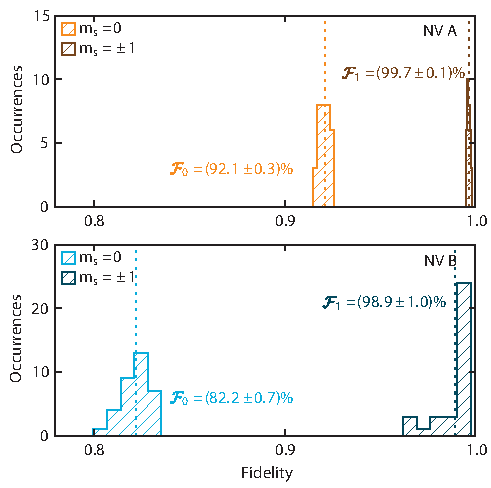
\includegraphics{ssro_histograms}
    \caption{Readout characterisation for both NVs. Imperfect spin-preparation before calibration measurements are taken into account. Histograms and means (red) of the SSRO fidelities, for both NVs, A and B, and both spin states, $\mszero$ and $\mspmone$, measured during all entanglement measurements.}
	\label{fig:ssrohist}
\end{figure}

\subsection{Maximum likelihood estimate of the state probabilities}
To estimate the eigenstate measurement populations $|c_{ij}|^2$ from a number of raw events $n_{ij}$ in which outcome $i$ has been obtained for NV A and outcome $j$ for NV B, we perform a maximum likelihood estimation.

The raw events are distributed according to a multinomial distribution $f(n_{ij})$ with parameters $p_{\uparrow\uparrow}$, $p_{\uparrow\downarrow}$, $p_{\downarrow\uparrow}$, and $p_{\downarrow\downarrow} = 1 - p_{\uparrow\uparrow} - p_{\uparrow\downarrow} - p_{\downarrow\uparrow}$, the probabilities for each possible outcome, that are in turn a function of the state probabilities $|c_{ij}|^2$, as defined from Eq.\,(\ref{eqn:ro_correction}) above.

The Likelihood function for the probabilities, parametrized by the measurement outcomes $n_{\uparrow\uparrow}$, $n_{\uparrow\downarrow}$, $n_{\downarrow\uparrow}, n_{\downarrow\downarrow}$, and $n = n_{\uparrow\uparrow} + n_{\uparrow\downarrow} + n_{\downarrow\uparrow} + n_{\downarrow\downarrow}$, is therefore
\be
\mathcal L\left[p_{ij}(E,|c_{ij}|^2)\right] = \frac{n!}{n_{\uparrow\uparrow}! n_{\uparrow\downarrow}! n_{\downarrow\uparrow}! n_{\downarrow\downarrow}!} p_{\uparrow\uparrow}^{n_{\uparrow\uparrow}} p_{\uparrow\downarrow}^{n_{\uparrow\downarrow}} p_{\downarrow\uparrow}^{n_{\downarrow\uparrow}} p_{\downarrow\downarrow}^{n_{\downarrow\downarrow}}.
\ee
The values $|c_{ij}|^2$ that maximise the likelihood are the desired populations. We verify that the found maxima are also global maxima by sampling through the parameter space numerically.

From the Likelihood function we also obtain Bayesian confidence intervals\cite{Lindsey:ub} (or credible intervals) by integration. We assume a uniform prior on the intervals $p_{ij}\in (0,1)$. The error bars in Fig.\,\ref{fig:rocorrection} and Fig.\,3 in the main text correspond to 68\% confidence intervals of the marginal probability distributions obtained from integrating over the two other probabilities. We note that the uncertainty originating form the uncertainty in the SSRO fidelities $\fid_{\uparrow,\downarrow}^\mathrm{A,B}$ is negligible compared to the statistical uncertainty.

\begin{figure}[h]
    \centering
    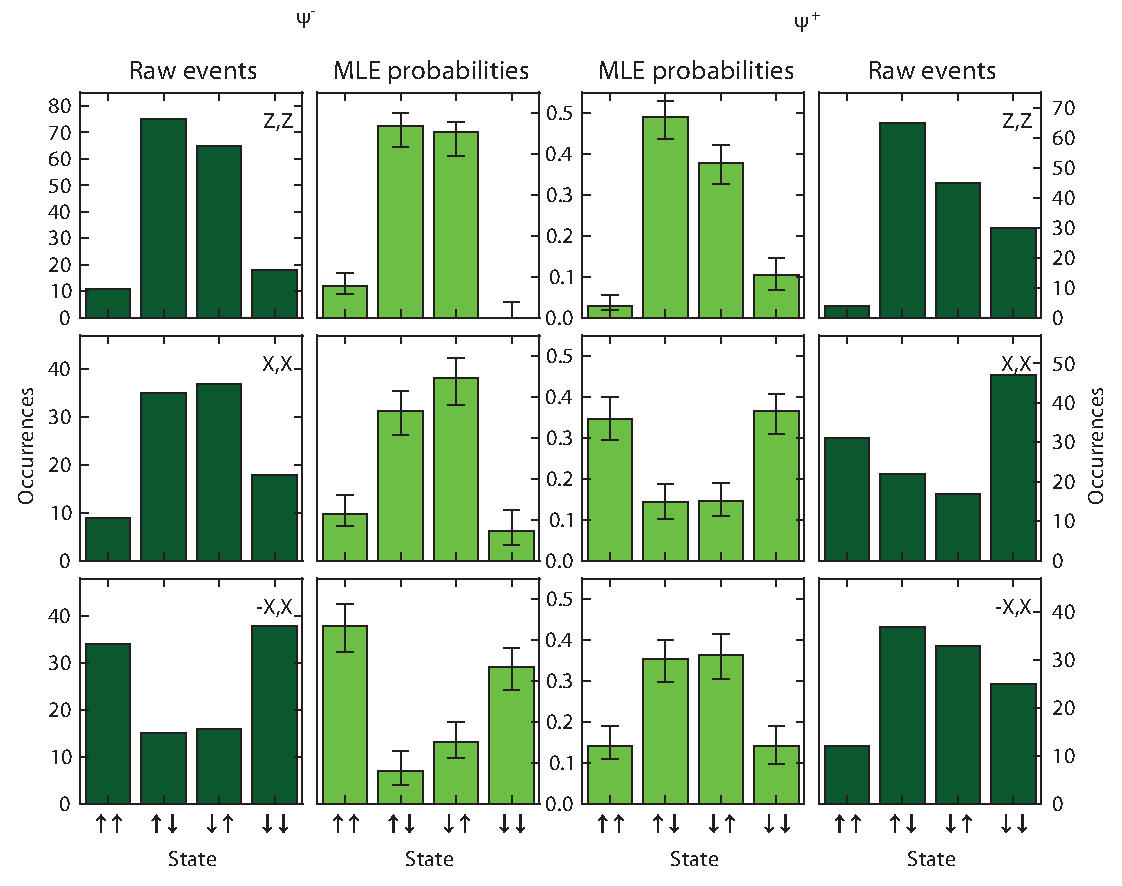
\includegraphics[width=12 cm]{fig_all_correlations.pdf}
    \caption{Raw events and MLE of the state populations $|c_{ij}|^2$, for both prepared states $\Psi^-$,$\Psi^+$, and all three measurement bases Z,Z; X,X; and -X,X as described in the main text. Each of the six subplots represents an independent MLE. We note that the MLE for the ZZ-basis measurement of $\Psi^-$ lies on the boundary of the physical space.}
	\label{fig:rocorrection}
\end{figure}

\subsection{Maximum likelihood estimate of the fidelity}

From the likelihood for a set of probabilities $p^\mathrm{Z,Z}_{ij}$ (for both spins measured in the Z-basis), $p^\mathrm{X,X}_{ij}$ (both spins measured in the X-basis) and $p^\mathrm{-X,X}_{ij}$ (spins measured in the X and $-\mathrm X$-basis, respectively), the likelihood for any value of $\fid$ can be obtained,
\be
\mathcal{L}(\fid) = \int_{\fid}\left ( \prod_{i,j}\mathrm dp^\mathrm{Z,Z}_{ij} \mathrm dp^\mathrm{X,X}_{ij} \mathrm dp^\mathrm{-X,X}_{ij} \right ) \mathcal L(p^\mathrm{Z,Z}_{ij}) \mathcal L(p^\mathrm{X,X}_{ij}) \mathcal L(p^\mathrm{-X,X}_{ij}),
\ee
where the integration is taken over a constant value of $\fid_\mathrm{LB}$ or $\fid$. The expression for $\fid_\mathrm{LB}$ is given in Eq.\,(\ref{eq:fidlowerbound}); for our best estimate for the fidelity, $\fid$, we set the square-root term in this expression to zero.

We perform this integration numerically (Fig.\,\ref{fig:fidemily}) for a set of values for $\fid_\mathrm{LB}$ and $\fid$. Because of the finite resolution of the numerical calculations, we fit the resulting distribution with a normalised Gaussian (free parameters are only the mean and the standard deviation) to obtain the best value and the 68$\%$ confidence interval, from the standard deviation of the Gaussian fit. Fig.\,\ref{fig:fidemily} shows that this procedure is justified for our results.

\begin{figure}[h]
    \centering
    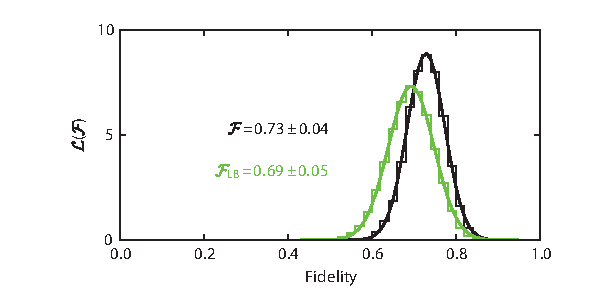
\includegraphics{emily}
    \caption{Maximum likelihood estimation for the state fidelity. We plot the likelihood density for resulting fidelities $\fid$ and $\fid_\mathrm{LB}$ for values spaced by 0.02. Thick lines are gaussian fits from which the means and standard deviations are obtained. Here we show the resulting distribution for $\Psi^-$, with a length of both detection windows of 38.4\,ns, and a maximal window for $|\delta \tau|$ of $25.6\,\text{ns}$.}
	\label{fig:fidemily}
\end{figure}


\section{Error estimation}
%Several sources of error lead to the observed reduction in fidelity with the desired Bell states. From independent measurements and simulations we estimate the following errors.

\subsection{Spin state initialization}
We initialise the electron spin of each NV in the $\mszero$ ground state by optical spin pumping on the $\ket{\mspmone}\leftrightarrow\ket{A_1}$ transition. The residual population in the $\mspmone$ states can be estimated from the fluorescence time-trace obtained during the pumping (Fig.\,\ref{fig:spinpumping}). With the initial fluorescence amplitude $A$ and the residual fluorescence level $y_0$, an upper bound for the remaining population in $\mspmone$ is given by $(y_0-y_{\mathrm{bg}})/(A+y_0-y_{\mathrm{bg}})$, where $y_{\mathrm{bg}}$ is the calibrated background level\cite{Robledo:2011fs}.

The fluorescence time-trace shows a clear double exponential behaviour with a fast component, on the order of a hundred nanoseconds, and a slower component on the order of microseconds. The fast timescale indicates a fast transition to a dark state that we attribute to the meta-stable singlet state.

\begin{figure}[h]
\centering
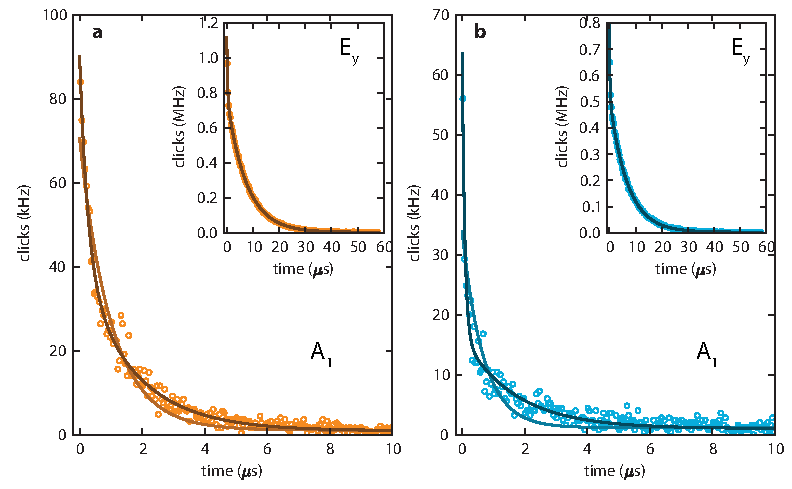
\includegraphics{spinpumping.pdf}
\caption{Fluorescence time-traces during spin pumping on the $\ket{\mspmone}\leftrightarrow\ket{A_1}$ transition for \textbf{a}, NV A and \textbf{b}, NV B. The laser power is the same as in the entanglement protocol and corresponds to near saturated driving. Insets show the curve for the $\ket{\mszero}\leftrightarrow\ket{E_y}$ transition (used for single-shot readout characterisation). The curves are fitted with a single-(light line) and double-(dark line) exponential decay with vertical offset. As can be seen the single exponential decay does not accurately describe the fluorescence for short time scales. From the double-exponential fits we obtain a total initial amplitude $A$ of $(89 \pm 2)$\,kHz and a offset $y_0$ of $(0.90 \pm 0.03)$\,kHz for NV A, and for NV B an amplitude $(62 \pm 1)$\,kHz and offset $(1.00 \pm 0.02)$\,kHz. Background $y_{\mathrm{bg}}$ for NV A,B is 350 Hz and 80 Hz respectively. From this we calculate an initialisation error of $(0.61 \pm 0.05)$\% for NV A and $(1.46 \pm 0.05)$\% for NV B. }
\label{fig:spinpumping}
\end{figure}

\subsection{Spin-flips in the excited state manifold}
During the two optical excitations in the entanglement protocol, a spin flip can occur due to spin-spin interactions in the excited state manifold. We can obtain an estimate of the probability of a spin-flip in the excited state, from the fluorescence time-trace of the used $E_y$ transition, given in the insets of Fig.\,\ref{fig:spinpumping}. Since this time-trace corresponds to driving near saturation, we can extract both the average number of photons detected $\langle n_{\text{detected}} \rangle = A_1 t_1 + A_2 t_2 $, and the detection efficiency $\eta = 2\frac{A_1+A_2}{\Gamma}$. Here, $A_1,t_1,A_1,t_2$ are the fit parameters obtained from the double exponential fit of the data and $\Gamma$ is the NV optical lifetime. From this we can calculate the average number of optical cycles $\langle n \rangle$ before a spin-flip occurs:
\be
\langle n \rangle = \frac{\langle n_{\text{detected}} \rangle}{\eta},
\ee
and finally, an estimate for the spin-flip probability per cycle $p_{\text{flip}}=\frac{1}{\langle n \rangle}$ of $0.46 \% \pm 0.01\%$ ($0.53\% \pm 0.01\%$) for NV A (NV B). We note that $p_{\text{flip}}$ corresponds to a crude estimate for the combined probability of a direct spin-flip due to spin mixing and a transition into the meta-stable single state. 

\subsection{Microwave Pulse Errors}
The fidelity of the microwave (MW) $\pi$ and $\pi/2$ pulses is limited by the static magnetic field applied and the hyperfine interaction with the NV host nitrogen nuclear spin. Because the nitrogen spin is not initialized, the MW pulses are randomly either on resonance or detuned by the hyperfine splitting of the \nfourteen ($2.2$\,MHz), depending on the state of the nitrogen spin. The error due to this detuning decreases with higher Rabi frequency. In the applied static magnetic field of 17.5 G, the $\mspone$ transition is 98 MHz detuned from the $\msmone$ transition. Therefore pulses with too high Rabi frequency will populate the $\mspone$ level. We drive Rabi oscillations for NV A of 10 MHz, and 8.6 MHz for NV B. For NV B we apply CORPSE pulses\cite{2003PhRvA..67d2308C} to reduce the effects of the detuning and to limit the population of the $\mspone$ level. For NV A we apply conventional pulses to avoid heating of the sample. We simulate the effect of the two errors on the combined state of the two NVs by numerically solving a three level driven system for the pulses used for each NV and calculating the $9\times9$ density matrix of the joint state. From this simulation we expect to reduce the fidelity of our final Bell State to 96.5$\%$  due to pulse errors. From the same simulation we find that the population of the $\mspone$ state is less than $0.4\%$ at the end of the protocol. The pulse simulations agree with independently measured $\pi$ pulse contrasts for both NVs.

\subsection{Spin Coherence and Dynamical Decoupling}
The main source of decoherence of the NV electron spins is the interaction with a spin bath of \cthirteen\ nuclear spins ($S = 1/2$). We measure a free induction decay time $T_2^{*}$ of ($3.07 \pm 0.06 $) $\mu$s for NV A and ($0.96 \pm 0.03$) $\mu$s for NV B. The spin echo of the electron spins periodically collapses and revives due to entanglement and disentanglement with the surrounding \cthirteen\ spins precessing in the external field\cite{Childress2006}. The revival amplitudes decay with a coherence time $T_2=687\,\mu\mathrm s$ (NV B).

For the dynamical decoupling we use a XY16 sequence\cite{Gullion:1990uj} and choose the inter pulse delay to be twice the Larmor period of the \cthirteen\ spins, thus measuring always the amplitude of the revivals. When applying more than 16 pulses, the pulse errors due to off-resonant driving of the $\mspone$ level become significant. To circumvent this limitation we initialize the \nfourteen\ nuclear spin by a projective measurement\cite{Robledo:2011fs}. This allows for a lower Rabi frequency (1.6 MHz) and therefore suppresses off-resonant driving of the $\mspone$ level.

\subsection{Residual laser photons}
After polarization rejection and time-filtering of the reflected laser photons there is still a finite probability of detecting a laser photon. Figure \ref{fig:laser_vs_nv} shows the combined count histogram during the first detection window on one APD, as well as the histogram counting only laser reflections, measured under similar conditions. With the chosen detection window settings there remains a $\sim 1\%$ probability that a detected photon comes from the laser instead of from either NV. Counting the possible two click events (NV+NV, NV+laser, laser+NV, laser+laser), this yields a 2\% probability for a fake heralding event. Assuming that fake heralding events actually correspond to totally mixed states in the $\mszero$, $\msmone$ subspace with $\fid=1/4$, this yields a state infidelity of 1.5\%.

\begin{figure}[h]
\centering
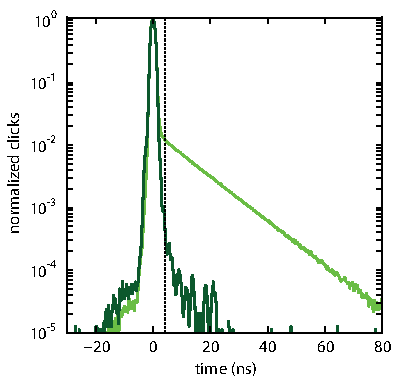
\includegraphics{laser_vs_NV.pdf}
\caption{To estimate the remaining laser photons in the time filtered signal we compare a time trace of the combined laser reflections and NV emission (light), and a time-trace showing only the laser pulse and reflections (dark). The NV data shown corresponds to the summed histogram of a single detector of the first excitation pulse of the whole entanglement dataset. The laser-only data was taken overnight under identical conditions, but with the excitation laser far detuned from the NV resonances. For both traces background is subtracted. The dashed line marks the start of the chosen detection window.}
\label{fig:laser_vs_nv}
\end{figure}


\subsection{Detector dark counts}
Our detectors have been selected for low dark counts, with an average dark count rate of less than 25 Hz. Taking into account the two detection windows and the probability of detecting a NV photon, we estimate a relative probability of 1.3\% for detecting a dark count. This yields a state infidelity of 2\%.

\subsection{Off-resonant excitation}
The 2\,ns optical $\pi$ pulses applied, have a small probability of exciting an off-resonant excited state transition. From Fig.\,2a in the main text it can be seen that the nearest transition corresponding to a $\msmone$ spin is detuned by $\sim 5\,\mathrm{GHz}$. We estimate the off-resonant excitation by simulating a 4-level driven system master equation in the Born-Markov approximation. Starting with an initial superposition of two ground states  corresponding to the $\mszero$, $\msmone$ levels, and two excited states corresponding to the resonantly driven $\mszero$ excited state level and the nearest off resonant $\mspmone$ level, we find a $\sim 1\%$ probability to excite the $\msmone$ state.

\subsection{APD After-pulsing}

With the APDs used in the experiment we observe after-pulsing, fake events that are triggered some time after the actual registration of a photon. In our entanglement scheme this can lead to fake heralding events: if a photon is detected in the detection window following the first laser pulse, there is a finite chance of obtaining a click on the same detector during the second detection not coming from a photon. Such events lower the fidelity of the produced entanglement. %In the case of such an event occurring, the impression will be left that the Bell state $\ket{\Psi^+}$ has been created, when in fact no entanglement has been generated.

We perform a control experiment to estimate the chance to detect such fake heralding events (Fig.\,\ref{fig:afterpulsing}). With the excitation laser strongly detuned from resonance we run the entanglement sequence, ideally (i.e., for no after-pulsing occurring) only expecting clicks from the laser reflection and background/dark counts. Identified after-pulsing events triggered by laser pulses are shown in Fig.\,\ref{fig:afterpulsing}a. To identify these events we assume that a click preceded by a click during a laser pulse is due to after-pulsing, neglecting the possibility of accidental double-events due to background/dark counts. This analysis implicitly includes erroneous entanglement heralding due to background/dark counts.

We obtain an estimate for the ratio of probabilities for real and fake heralding of $\Psi^+$ generation as follows. We compare the probability for detecting an NV photon after excitation by the second laser pulse in the entanglement measurement and the probability for registering during the same window an after-pulsing event triggered by the first laser pulse (Fig.\,\ref{fig:afterpulsing}b). For fake heralding events the after-pulsing event is triggered by an NV photon. Therefore, after-pulsing events are expected later than those triggered by the laser. We neglect this time-difference because the probability for an after-pulsing event during the detection window is almost constant.

\begin{figure}[h]
    \centering
    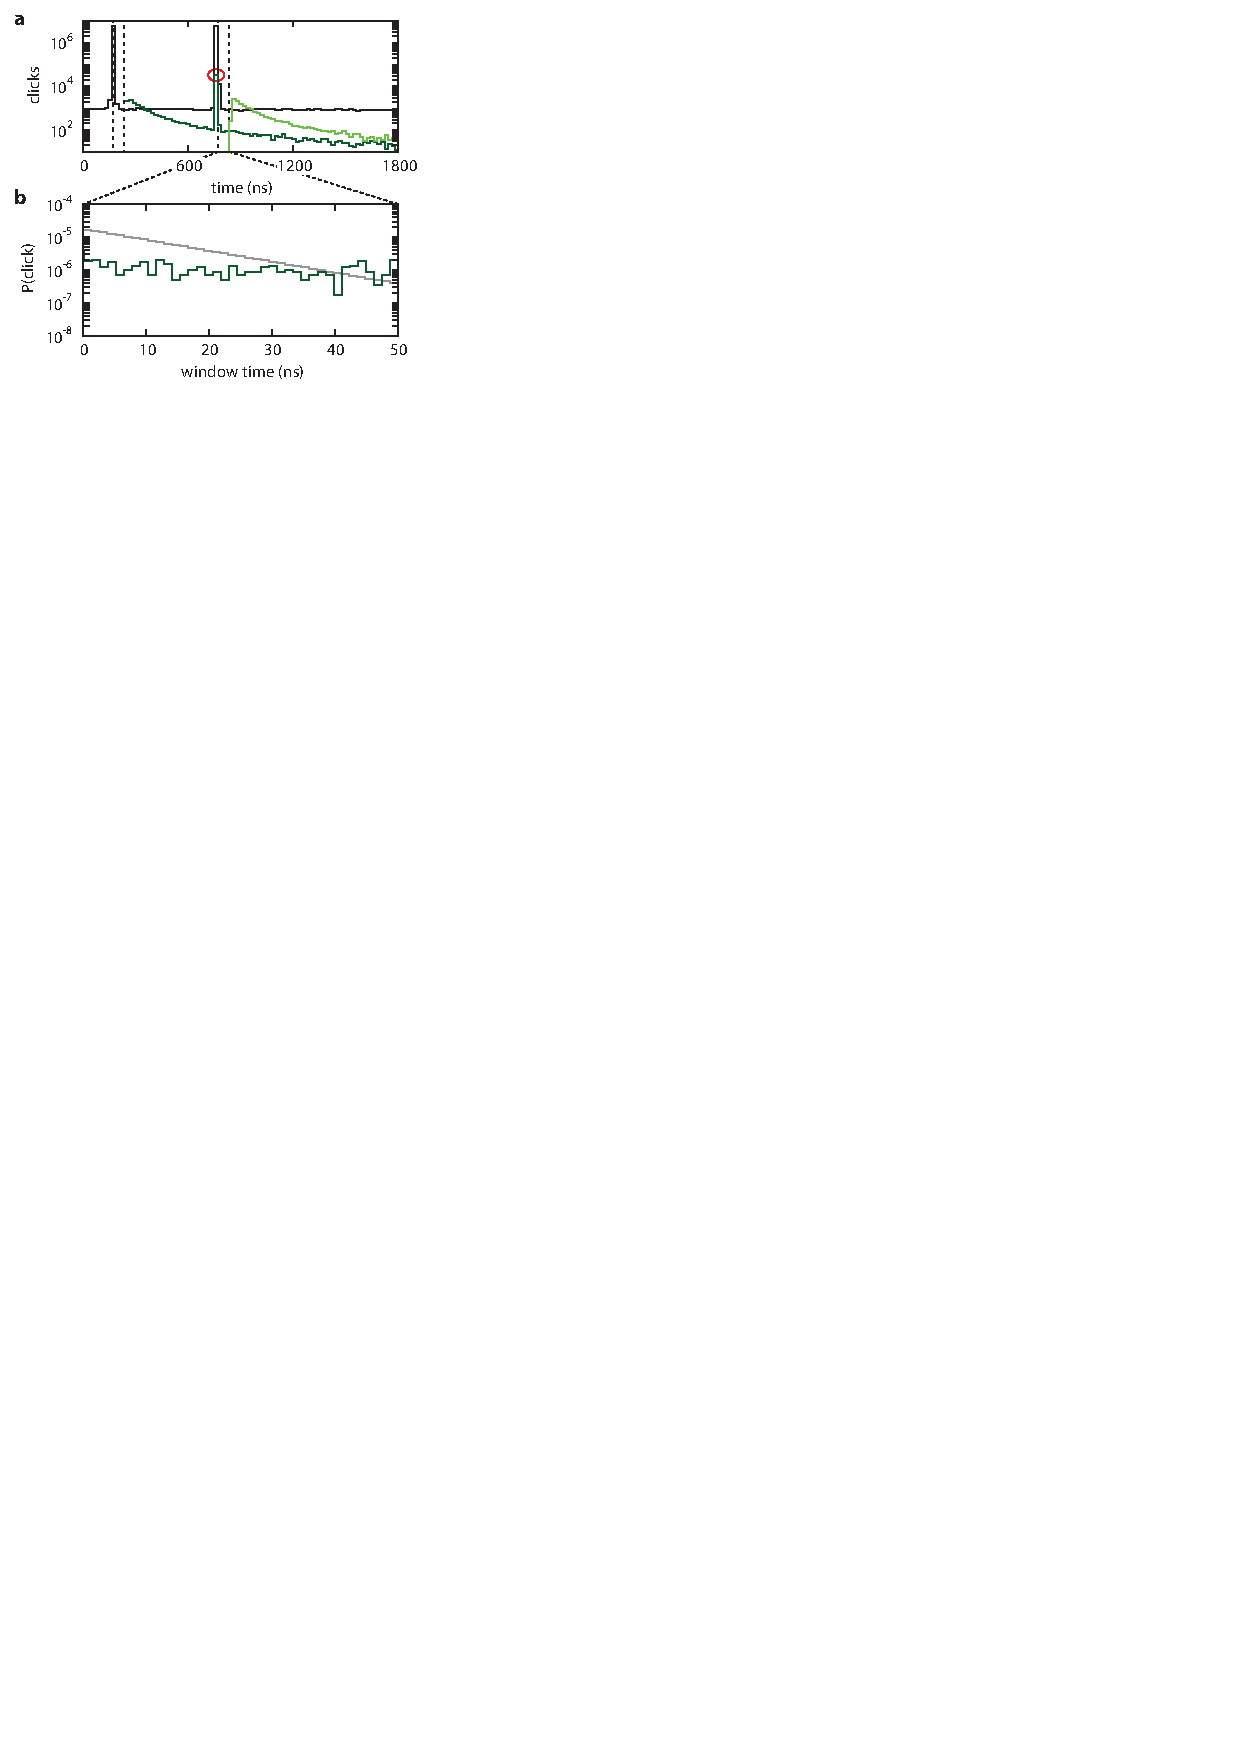
\includegraphics[clip=true,trim=0cm 23cm 13.8cm 0cm]{afterpulsing}
    \caption{After-pulsing. \textbf{a}, After-pulsing events following laser pulses, measured on one APD after the beam splitter. We identify detection events (green histogram curves) that are registered after a laser photon from the first and second laser pulse, respectively. The black curve shows events that are not preceded by another detection event (laser photons and dark/background counts). Dashed lines mark the range used to identify entanglement events. The high probability for a click obtained during the second laser pulse after obtaining a click during the second (data point encircled red) is not due to after-pulsing but due to the comparatively high probability of detecting a photon from both pulses in the same run. \textbf{b}, Detection probabilities for NV photons and after-pulsing events. The green curve shows the probability to detect in the second detection window an after-pulsing event triggered by the first laser pulse. The grey curve shows for comparison the typical probability to detect an NV photon.}
	\label{fig:afterpulsing}
\end{figure}

For the chosen detection window of 19.2\,ns after the second excitation we find an 8.8\% relative probability to measure an afterpulsing event instead of an NV photon. Assuming that fake heralding events actually correspond to totally mixed states in the $\mszero$, $\msmone$ subspace with $\fid=1/4$, this leads to an infidelity of 6.5\%. Note that this error only applies for the $\Psi^+$ state.

%In the analysis presented in Fig.\,4 of the main text we include the dependence of the after-pulsing on the relative photon delay. Because the after-pulsing probability is approximately constant in time (Fig.\,\ref{fig:afterpulsing}b), it is not dependent on the delay $\delta \tau = \tau_2 - \tau_1$, where $\tau_1$ ($\tau_2$) is the detection time after the first (second) laser pulse. However, the probability for a real entanglement event with delay $\delta \tau$ is determined by the exponentially decaying probabilities to detect NV photons after both excitation pulses. Therefore, the probability that an entanglement event is real depends on $\delta \tau$.

%The probability density function (PDF) for a real entanglement event with delay $\delta \tau$ after having registered the first photon at time $\tau_1$ is given by 
%\be
%P(\delta \tau \mid \tau_1) \propto \mathrm e^{-\Gamma(\tau_1 +\delta \tau)},\hspace{1em} \delta \tau \geq -\tau_1.
%\ee
%The PDF for all possible $\tau_1$ is then obtained by integration, taking into account the pulse starts and detection windows of %lengths $w_1$ and $w_2$,
%\be
%P(\delta \tau) \propto \int_0^{w_1} \mathrm d\tau_1 \mathrm e^{-\Gamma \tau_1} \mathrm e^{-\Gamma(\tau_1 +\delta \tau)} %\Theta(\delta \tau+\tau_1) \Theta(w_2 - \delta\tau - \tau_1),
%\ee
%where $\Theta$ is the Heaviside step function. This allows us to calculate $P(real photon)(\delta \tau)

\subsection{Dephasing}
The largest contribution to the state infidelity is dephasing of the produced Bell state due to distinguishability of the photons emitted by the NV centres. An estimate for the distinguishability of the photons can be gained from the two-photon interference presented in figure 2d of the main text. The interference shows a reduced visibility due to distinguishability of the photons. As explained in more detail in the section on phase evolution below, the visibility $V$ gives an upper bound for the Bell state fidelity:
$\fid\leq 1/2 + 1/2 V$.

The photon distinguishability is likely caused by phonon-induced transitions between optically excited states, mainly in NV A, which is operated at a higher temperature. Another contribution is the resonance check performed before the entanglement protocol to ensure both NV's are on resonance: to minimize the time necessary for the resonance check, the NV's are excited with a laser power near saturation. This can however decrease the frequency-selectivity of the resonance check, as the lines will be power broadened.
%For a typical detection time window, this yields an upper bound of This is explained in more detail in section \ref{sec:phases} below.% the indistinguishably is quantified an related to the maximal obtainable fidelity. XXX%However, laser reflections and dark counts can also reduce the visibility. To estimate the error solely due to dephasing effects, we can use measurements of the inhomogeneously broadened emission line-widths of the NV centres, such as the laserscans presented in figure 2a of the main text and the optical Rabi-oscillations in figure XX. From these we get a Gaussian distribution of the emission frequencies with a width of XX MHz. We can average the fidelity obtained in section XX for the overlap with the desired bell state over these emission frequencies. Taking into account the exponential decay of the emission probability in both time windows, we then find a maximum fidelity overlap due to dephasing of F=0.78.  Note that this error only shows in the rotated basis measurements.

\section{TPQI signature}

As a measure of the indistinguishability of the photons from NV A and B we evaluate the difference between the measured $g^{(2)}(dt)$ function and the expected function $g^{(2)}_\perp(dt)$ that would be obtained in the case of perfectly distinguishable photons. We define the visibility as
\be
	\label{eqn:tpqi_visibility}
	V(dt) = \frac{g^{(2)}_\perp(dt) - g^{(2)}(dt)}{g^{(2)}_\perp(dt)}.
\ee

$g^{(2)}(dt)$ is proportional to the histogram of all coincidences obtained between photons detected on the two APDs after the beam splitter, where $dt = t_1 - t_2$, and $t_1$ ($t_2$) is the arrival time of the photon detected by APD 1 (2). We only take into account photons obtained during the same entanglement attempt. Because our pulse scheme consists of two optical $\pi$ pulses, coincidence peaks only occur around $dt = 0\,\text{ns}$ (two photons detected after the same excitation pulse) and $dt = \pm 600\,\text{ns}$ (one photon detected after each excitation pulse). 

To determine $g^{(2)}_\perp(dt)$ from our measurement we can use the coincidence count-rates of the side peaks around $dt = \pm 600\,\text{ns}$. The shape of $g^{(2)}_\perp(dt)$ for two single emitters in our pulse scheme is given by
\be
g^{(2)}_\perp(dt) = \sum_{i=-1,0,1} A_i \exp (-\Gamma |dt - i\times 600\,\text{ns}|),
\ee
where the relative amplitudes $A_i$ are determined by the spin-dependent excitation probabilities: The full state of the system after the first excitation round has the form (see main text)
\be
	\ket{\psi} = \frac{1}{2} \left ( \ket{\uparrow\uparrow}\ket{11} +  \ket{\downarrow\downarrow}\ket{00} + \ket{\uparrow\downarrow}\ket{10} + \ket{\downarrow\uparrow}\ket{01} \right ).
\ee
Neglecting initialisation and microwave errors, the $\ket{00}$, $\ket{11}$ states both contribute to the $A_0$ peak only, and the $\ket{01}$, $\ket{10}$ states contribute to the $A_{\pm 1}$ peaks only. Because all states occur with equal probability ($1/4$) and collection efficiency factor ($\eta_A\eta_B)$, we have 
\be
A_0=A_{-1}+A_{+1} \text{, and }A_{-1}=A_{+1}.
\ee
The amplitudes $A_{\pm 1}$ can be extracted from the measurement of $g^{(2)}(dt)$, because for the side peaks, $g^{(2)}(dt) = g^{(2)}_\perp(dt)$. %(Here no interference is possible because the photon wave-packets do not overlap in time XXX.)

We note that in Fig.\,3 of the main text we have renormalised the central peak such that $g^{(2)}_\perp(0\,\text{ns}) = 1/2$, the expected result for a conventional pulsed TPQI experiment, with an infinite pulse sequence and two single emitters, for clarity. As the same normalisation factor is applied to the measured central peak of $g^{(2)}(dt)$, this does not change the visibility.%XXXX


\section{Phase of the entangled state}
\label{sec:phases}
Considering all relevant phases, the quantum state of the system after the first excitation before the beam splitter is
\begin{align}
&\frac{1}{2} \left[ (e^{-i \omega_{\downarrow}^A t}\ket{\downarrow}_A\ket{0}_A + e^{-i \omega_{\uparrow}^A t}\ket{\uparrow}_A e^{i k_A x_A -i \omega_A \tau}\ket{1}_A)\right.\\ \nonumber
&\left . \qquad \otimes (e^{-i \omega_{\downarrow}^B t}\ket{\downarrow}_B \ket{0}_B - e^{-i \omega_{\uparrow}^B t}\ket{\uparrow}_B e^{i k_B x_B -i \omega_B \tau}\ket{1}_B)\right],
\end{align}
where $\omega_{\downarrow_i}$ and $\omega_{\uparrow_i}$ correspond to the energy levels for the two ground states $\{\ket{\downarrow},\ket{\uparrow}\}$. $\omega$ is  the transition frequency from the excited state $\ket{e}$ to the corresponding ground state and $k$ the corresponding wavenumbers $k=\omega/c$. $x$ is the photon path length from the NV-centre to the beam splitter, the time $t$ corresponds to the time after the first MW $\pi/2$ pulse and time $\tau$ to the time after the excitation pulse. The labels $\{A,B\}$ denote the two NV centres. See also Fig.\,\ref{fig:levels}.

\begin{figure}[h]
\centering
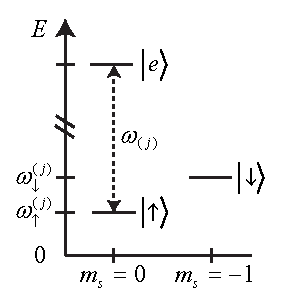
\includegraphics[width=3.5cm]{levels_short.pdf}
\caption{Schematic showing the energy levels involved in the protocol, and the definitions for the various frequencies $\omega$ involved, where $j$ labels the NV centre $j\in \{\text{A,B}\}$}.
\label{fig:levels}
\end{figure}

After a single click in one of the output ports of the beam-splitter at a time $\tau_1 > k_A x_A, k_B x_B$ after the excitation (caused by one or two photons in that port), the two NV spins are projected onto the mixed state
\begin{equation}
\label{eqn:mixed_state}
|\alpha|^2 \ket{\psi^{\pm}}_{AB} \bra{\psi^{\pm}}_{AB} + |\beta|^2  \ket{\uparrow}_A\ket{\uparrow}_B\bra{\uparrow}_A\bra{\uparrow}_B,
\end{equation}
with the $(-)$-sign if we detect a click on the detector on output port 1 and a $(+)$ for a click on 2, and amplitudes $\alpha, \beta$ depending on the collection efficiencies for NV A and B, respectively. $\ket{\psi^{\pm}}_{AB}$ is an entangled state, with, at time $t_{MW}$ after the first MW $\pi/2$-pulse, the following phase relations:
\begin{align}
\nonumber
\label{eqn:phases_round_1}
\ket{\psi^{\pm}}_{AB}&=\frac{1}{\sqrt{2}}\left[ e^{-i\omega_\downarrow^A t_{MW}} \ket{\downarrow}_A e^{-i\omega_\uparrow^B t_{MW}} \ket{\uparrow}_B \cdot e^{i k_B x_B - i \omega_B \tau_1} \right. \\ 
& \qquad \qquad \left. 
\pm \quad e^{-i\omega_\uparrow^A t_{MW}} \ket{\uparrow}_A e^{-i\omega_\downarrow^B t_{MW}} \ket{\downarrow}_B \cdot e^{i k_A x_A - i\omega_A\tau_1} \right].
\end{align}
Here we have assumed identical NV-optical lifetimes $\Gamma^{-1}$ and identical path-lengths from the beam splitter to the two different detectors, for simplicity.

At this time, the MW $\pi$-pulse is applied, flipping all $\ket{\downarrow} \longleftrightarrow \ket{\uparrow}$ in Eqns.\,(\ref{eqn:mixed_state}), (\ref{eqn:phases_round_1}). Then the second excitation round proceeds, and after again detecting a single click in one of the output ports of the beam-splitter at a time $\tau_2 > k'_A x'_A, k'_B x'_B$, the two NV spins are projected onto the pure state:
\begin{align}
\label{eqn:total_phase}
\nonumber
&\frac{1}{\sqrt{2}}\left[ e^{-i\omega_\downarrow^A t_{MW}} e^{-i\omega_\uparrow^{' A} t_{MW}} \ket{\uparrow}_A e^{-i\omega_\uparrow^B t_{MW}} e^{-i\omega_\downarrow^{' B} t_{MW}} \ket{\downarrow}_B \right. \\ \nonumber
& \qquad \qquad \left. \times \quad e^{i k_B x_B -i \omega_B\tau_1} e^{i k'_A x'_A- i \omega'_A \tau_2}\right. \\ \nonumber
& \qquad  \left. 
\pm \quad e^{-i\omega_\uparrow^A t_{MW}}e^{-i\omega_\downarrow^{' A} t_{MW}} \ket{\downarrow}_A e^{-i\omega_\downarrow^B t_{MW}}e^{-i\omega_\uparrow^{' B} t_{MW}} \ket{\uparrow}_B \right. \\ 
& \qquad \qquad \left. \times \quad e^{i k_A x_A -i\omega_A \tau_1} e^{i k'_B x'_B - i \omega'_B \tau_2} \right],
\end{align}
at the spin-echo time $t=2 \times t_{MW}$ after the first MW $\pi/2$-pulse. Here we have denoted variables corresponding to physical quantities during the second round with a prime ('). The ($+$)-sign corresponds to a click in the same detectors, the ($-$)-sign to different detectors.

The phase of the final entangled in Eq.\,(\ref{eqn:total_phase}) contains terms that oscillate with the photon frequency. To produce useful entanglement, a stable phase is required, suggesting that spatial interferometric stability of the setup and prohibitively small detector time jitter are needed. 

However, the time $T$ between the two excitation rounds is short ($T=600$\,ns) compared to many environmental drifts of e.g. the optical path lengths and electric and magnetic fields. This suggests we should consider certain assumptions about the relation between the physical quantities in the first and second excitation rounds. In particular, possible assumptions are:

\begin{enumerate}
\item $\omega_\uparrow = \omega_\uparrow'$ and $\omega_\downarrow=\omega_\downarrow'$, requiring stability of the magnetic field as felt by the NV centre on the time-scale $T$. From independent spin-echo measurements in e.g. figure 1b in the main text we know that this assumption satisfied.
\item $x=x'$ requiring stability of the setup on the order of a wavelength (637\,nm) on the time-scale $T$. With $T$ being only 600ns, the setup is expected to be stable. 
\item $\omega=\omega'$ (and therefore also $k=k'$). This assumption is harder to justify by independent measurement, and in fact would not be satisfied if phonon-induced transitions occur in the excited state. %Nonetheless, a comparison can be made between the resulting expression for the state fidelity and the TPQI visibility, as explained in the section below.
\end{enumerate}

If all three assumptions are satisfied, the phase relation in Eq.\,(\ref{eqn:total_phase}) simplifies: 
\begin{equation}
\frac{1}{\sqrt{2}}\left(\ket{\downarrow\uparrow}_{AB} \pm e^{i\varphi} \ket{\uparrow\downarrow}_{AB}\right),
\end{equation}
with
\begin{equation}
\label{eqn:phase_deph}
\varphi(\tau_1,\tau_2) = (\tau_2-\tau_1)(\omega_A - \omega_B),
\end{equation}
so that the overlap with the wanted Bell states is:
\begin{equation}
\label{eqn:fid_deph}
F(\varphi)= \frac{1}{2}+\frac{1}{2}\cos(\varphi).
\end{equation}

This analysis shows that whenever the two NV centers are on resonance, perfect state fidelity could be obtained independent of the photon arrival times. Also, if the photon arrival times are identical, no dephasing is present independent of the detuning between the NV centers' optical frequencies.

\subsection{Relation to TPQI visibility}
Following Legero \emph{et al.}\cite{Legero:2006ur}, we have for the two-photon correlation function $g^{(2)}(t_1,t_2)$ of two photons with identical polarisation exiting from the beam-splitter:
\begin{equation}
	g^{(2)}(t_1,t_2)=\frac{1}{4}\left|\xi_A(t_1)\xi_B(t_2)-\xi_B(t_1)\xi_A(t_2)\right|,
\end{equation}
where $\xi(t)$ describes the spatio-temporal mode of the state of a single-photon light field, at time $t$. When these modes are written as the product of a real amplitude and a complex phase, $ \xi_i(t) = \epsilon_i(t) \exp[ - i \phi_i(t)]$, the correlation above function can be rewritten:
\begin{equation}
	g^{(2)}(t_1,t_2)=g^{(2)}_\perp(t_1,t_2) - K(t_1,t_2).
\end{equation}
Here, $g^{(2)}_\perp(t_1,t_2)$ is the correlation function for two fully distinguishable (perpendicularly polarised) single photons,
\begin{equation}
g^{(2)}_\perp(t_1,t_2) = \frac{1}{4}\left((\epsilon_A(t_1)\epsilon_B(t_2))^2 + (\epsilon_A(t_2)\epsilon_B(t_1))^2 \right),
\end{equation}
which is independent of the phases $\phi$. $K(t_1,t_2)$, however, does depend on the phase:
\begin{equation}
K(t_1,t_2) = \frac{1}{2}(\epsilon_A(t_1) \epsilon_B(t_2) \epsilon_A(t_2) \epsilon_B(t_1))\cos(\phi_A(t_1)-\phi_A(t_2) + \phi_B(t_2) - \phi_B(t_1)).
\end{equation}
Finally, the visibility of the two photon interference in Eq.\,(\ref{eqn:tpqi_visibility}) is given by %$V(\tau)=\int_0^{t_{\text{max}}}\delta t'v(t',t'+\tau)$ with
\begin{equation}
V(t_1,t_2)=\frac{g^{(2)}_\perp-g^{(2)}}{g^{(2)}_\perp}= K/g^{(2)}_\perp.
\end{equation} 

Relating the above to photons emitted by our two NV centres in the situation in our experiment, and assuming the excitation time $t_0$, we have
\begin{equation}
\epsilon_i(t)=\Gamma\exp[\Gamma(t-t_0-x_i/c)],
\end{equation}
where we have assumed as before identical optical lifetime $\Gamma^{-1}$ for the both NV's. Furthermore:
\begin{equation}
\phi_i(t)=(t-t_0)\omega_i-k_i x_i.
\end{equation}
In this case, $V(t_1,t_2)$ above reduces to 
\begin{equation}
V(t_1,t_2)=\cos[(t_2-t_1)(\omega_A-\omega_B)].
\end{equation}

Comparing this result with Eqns. (\ref{eqn:phase_deph}),(\ref{eqn:fid_deph}) above, we have $\frac{1}{2} + \frac{1}{2}V(dt)=F(\varphi(\delta\tau))$, with - as before - $dt=t_2-t_1$ and $\delta \tau = \tau_2-\tau_1$. Since rejecting any of the assumptions (1-3) made in the previous section to arrive at the simplified expression for $F$ will in general decrease the fidelity, $V$ sets an upper limit for the fidelity overlap with the Bell states.


\newpage
\bibliographystyle{../thesis}
\bibliography{lde_appendix}


